\chapter{Orderbook Agents}
This chapter describes several \emph{Orderbook Agents}, implemented to learn optimal \emph{Submit \& Revise} trading strategies from a given training data set.


\section{Implementation}
\label{chap:experiments:implementation}
Each \emph{Orderbook Agents} inherits some commonly shared functionality from the super class \lstinline!class RL_Agent_Base!. This base class provides a consistent framework, allowing to swap the logic behind \lstinline!learn_from_samples! and \lstinline!predict! only, while general functionality like \lstinline!load!, \lstinline!save!, \lstinline!plot_heatmap_Q! and \lstinline!collect_samples! may be reused.



\subsection{Backward Sampling \& Learning}
The process of sampling from training data and learning optimal state-action values has been split into two independent phases, mostly due to performance\footnote{The backward sampling phase for the example mentioned in \Cref{chap:backwardlearning}, took roughly 10 hours, even though the work load was distributed among 24 CPU's.} reasons. In the \emph{sampling phase}, all possible combinations of actions and private variables are evaluated and stored as 5-tuples $sample=(state, action, cost, timestamp, new\_state)$. As market variables are supposedly not influenced by the agents behavior (see \Cref{chap:statespace}), it suffices to remember the orderbooks time point, to allow adjacent substitution of market variables.\\

Samples are stored as DataFrame and may be exported and reused by other agents, as wished. This allows to skip the time consuming process of backward sampling. Before the action learning phase starts, the collected samples may be enhanced by a variety of market variables, discretized or untouched. The helper function \lstinline!addMarketFeatures_toSamples()! retrospectively adds market variables to the agents samples DataFrame.\\

If wanted, features are discretized according to their individual value range.\\
\Eg a chosen resolution of 3, evenly transforms features $o_m$ into $o_{m\_disc3}$, according to automatically determined boundaries: \\
0 (if $o_m< 1/3$ quantile), 1 (if $1/3 \leq o_m < 2/3$ quantile) and 2 (if $o_m \geq 2/3$ quantile). Quantiles come from the training data and are applied to test data unaltered.\\

The learning phase starts hereinafter, whereas three types of orderbook agents have been implemented and experimented with, each of which employs different techniques:

\begin{description}
\item[QTable\_Agent] : Dynamic Programming as described in \Cref{chap:backwardlearning}.\\
Expected state-values are stored in a simple lookup table, hence discretization of the state space is required. For each state, a vector of length $L=num\_actions$ is maintained, of which the first argmin refers to the optimal action. The \emph{QTable} does not generalize to previously unobserved states and returns the very first action (here -4) in such a case. For proper cost-updates an additional \emph{NTable} is maintained, referencing the number of observations made.\\
QTable and NTable entries are computed in an iterative manner. In the first round, all samples with \lstinline!time_left=1! are evaluated, in the second round all samples with \lstinline!time_left=2!, \etc The private variable \lstinline!volume! is discretized according to the specified resolution and linear cost scaling, as described in \Cref{chap:backwardalgorithm:discussion:costscaling}, is performed.

\item[BatchTree\_Agent]: Tree-Based Batch Mode Reinforcement Learning \Cite{Ernst:2005:TreeBasedBatchModeRL}.\\
An ensemble of 100 decision trees, with a maximum allowed depth of 20 is fed with the full batch of samples simultaneously, no discretization require. $T*2$ learning rounds are performed, to completely allow expected costs to unfold over the given time horizon.\\
The state space is enlarged by an extra dimension for the chosen action. Predicting the optimal action to choose for a given state, the ensemble must be queried $L=num\_actions$ times, from which the argmin refers to the optimal action.

\item[NN\_Agent] : Neural fitted Q Iteration \Cite{Riedmiller:2005:NFQ}.\\
A simple multi layer perceptron with 400 hidden units and 1 output neuron is trained in mini batches of size 4.096, optimized over multiple epochs by Adam\Cite{Kingma:2014:Adam} with a learning rate of 0.01. As with the BatchTree\_Agent, no state space discretization is required and actions are included into the state space and $L$ predictions are required, to obtain the optimal action.
\end{description}



\subsection{Forward Sampling \& Learning}
In order to create more realistic orderbook shapes (see \Cref{chap:backwardalgorithm:discussion:markovianassumption}), an forward sampling method is presented.


\begin{lstlisting}[frame=single, breaklines=true, basicstyle=\scriptsize, caption=Forward sampling approach., label=lst:forward:pseudocode]
collect_samples_forward(V, H, T, I, L, E)
    While(not end of data)
        init OTS with V=100%
            For epoch=0 to E
                reset OTS at random startpoint
	            Transform (orderbook) -> o_1 ... o_R
	            Apply e-greedy strategy until V=0%
		    Store samples in DataFrame
		    
\end{lstlisting}




\section{Experiments}
\label{chap:experiments}
\subsection{Action-Limit Mapping}
\label{chap:exp:actionlimitmapping}
As mentioned in \Cref{chap:backwardalgorithm:discussion:actionspace}, it seems pointless to force actions to cross the bid-ask-spread before any orders can be matched. \Cref{fig:actionlimitmapping} compares strategies learned from differing limit base levels.

\begin{figure}[ht]
	\centering
	
	\begin{subfigure}[b]{0.7\textwidth}
        		\centering
        		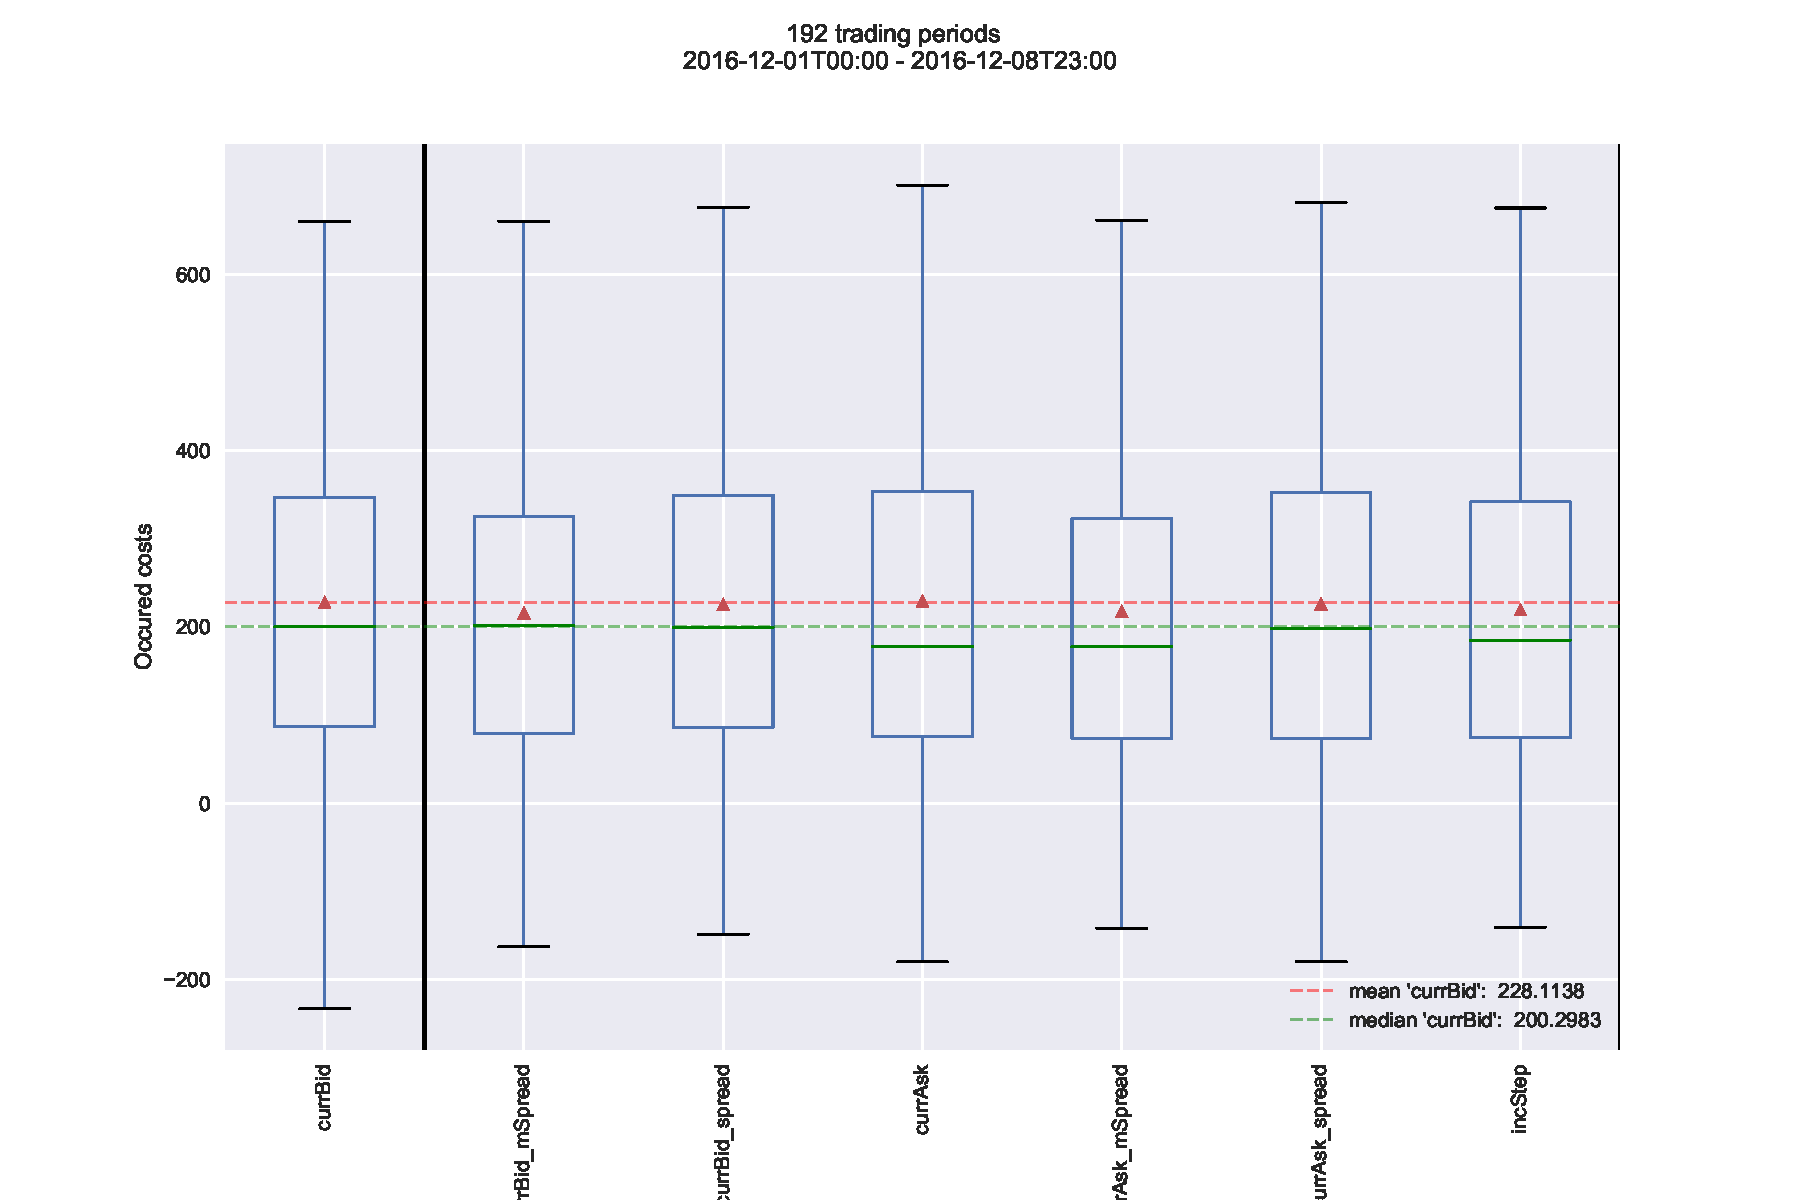
\includegraphics[width=\textwidth]{content/drawings/performance_limitBase_dec.pdf}
        		\caption{Slippage.}
		\label{fig:actionlimitmapping:plot}
    	\end{subfigure}%
	\begin{subfigure}[b]{0.30\textwidth}
        		\centering
		\scalebox{0.7}{
\begin{tabular}{lr}
\toprule
{} &           mean slippage \\
\midrule
currBid         &  228.11 \\
currBid\_mSpread &  215.90 \\
currBid\_spread  &  225.99 \\
currAsk         &  229.11 \\
currAsk\_mSpread &  217.88 \\
currAsk\_spread  &  226.12 \\
incStep         &  219.48 \\
\bottomrule
\end{tabular}	
		}  \vspace{1.8cm}      		 
        		\caption{Mean slippage.}
		\label{fig:actionlimitmapping:mean}
    	\end{subfigure}

	\caption{Evaluating the impact of additional market variables.}
	\label{fig:actionlimitmapping}
\end{figure}

Throughout the rest of this thesis, the same 15 actions are evaluated: $[-4, -3, ..., 8, 9, 10]$, corresponding to limit factors of $[0.996, 0.997, ..., 1.008, 1.009, 1.01]$\\




\begin{itemize}
\item actions represent deviation from ask, not bid
\item Forward Sampling
\begin{itemize}
\item Growing batch learning
\item Experience Replay (NN\_Agent)
\item Exploration vs avoidance of repeatedly trying same actions.
\end{itemize}
\begin{itemize}
\item Markov Property violated
\item Realistic samples, no rounding. Better fit for \emph{curious} masterbook shapes as described in \Cref{chap:modelcorrectness}?!
\end{itemize}
\item Function Approximation
\begin{itemize}
\item RandomForest (BatchTree Agent)
\item NN Agent
\end{itemize}
\item Different Market Variables:
\begin{itemize}
\item Immediate Slippage/MarketPrice Imbalance
\item MarketPrice Spread (buy vs. sell)
\end{itemize}
\item Cost function
\begin{itemize}
\item Slippage based on initial\_center
\item Improvement over MarketPrice??
\end{itemize}
\end{itemize}


\section{RL Agents}
bla

\subsection{QTable Agent}
bla

\subsection{BatchTree Agent}
bla

\subsection{NN Agent}
bla



\section{Additional Market Variables}
\label{chap:exp:additionalmarketvars}





\begin{figure}[ht]
	\centering
	
	\begin{subfigure}[b]{0.6\textwidth}
        		\centering
        		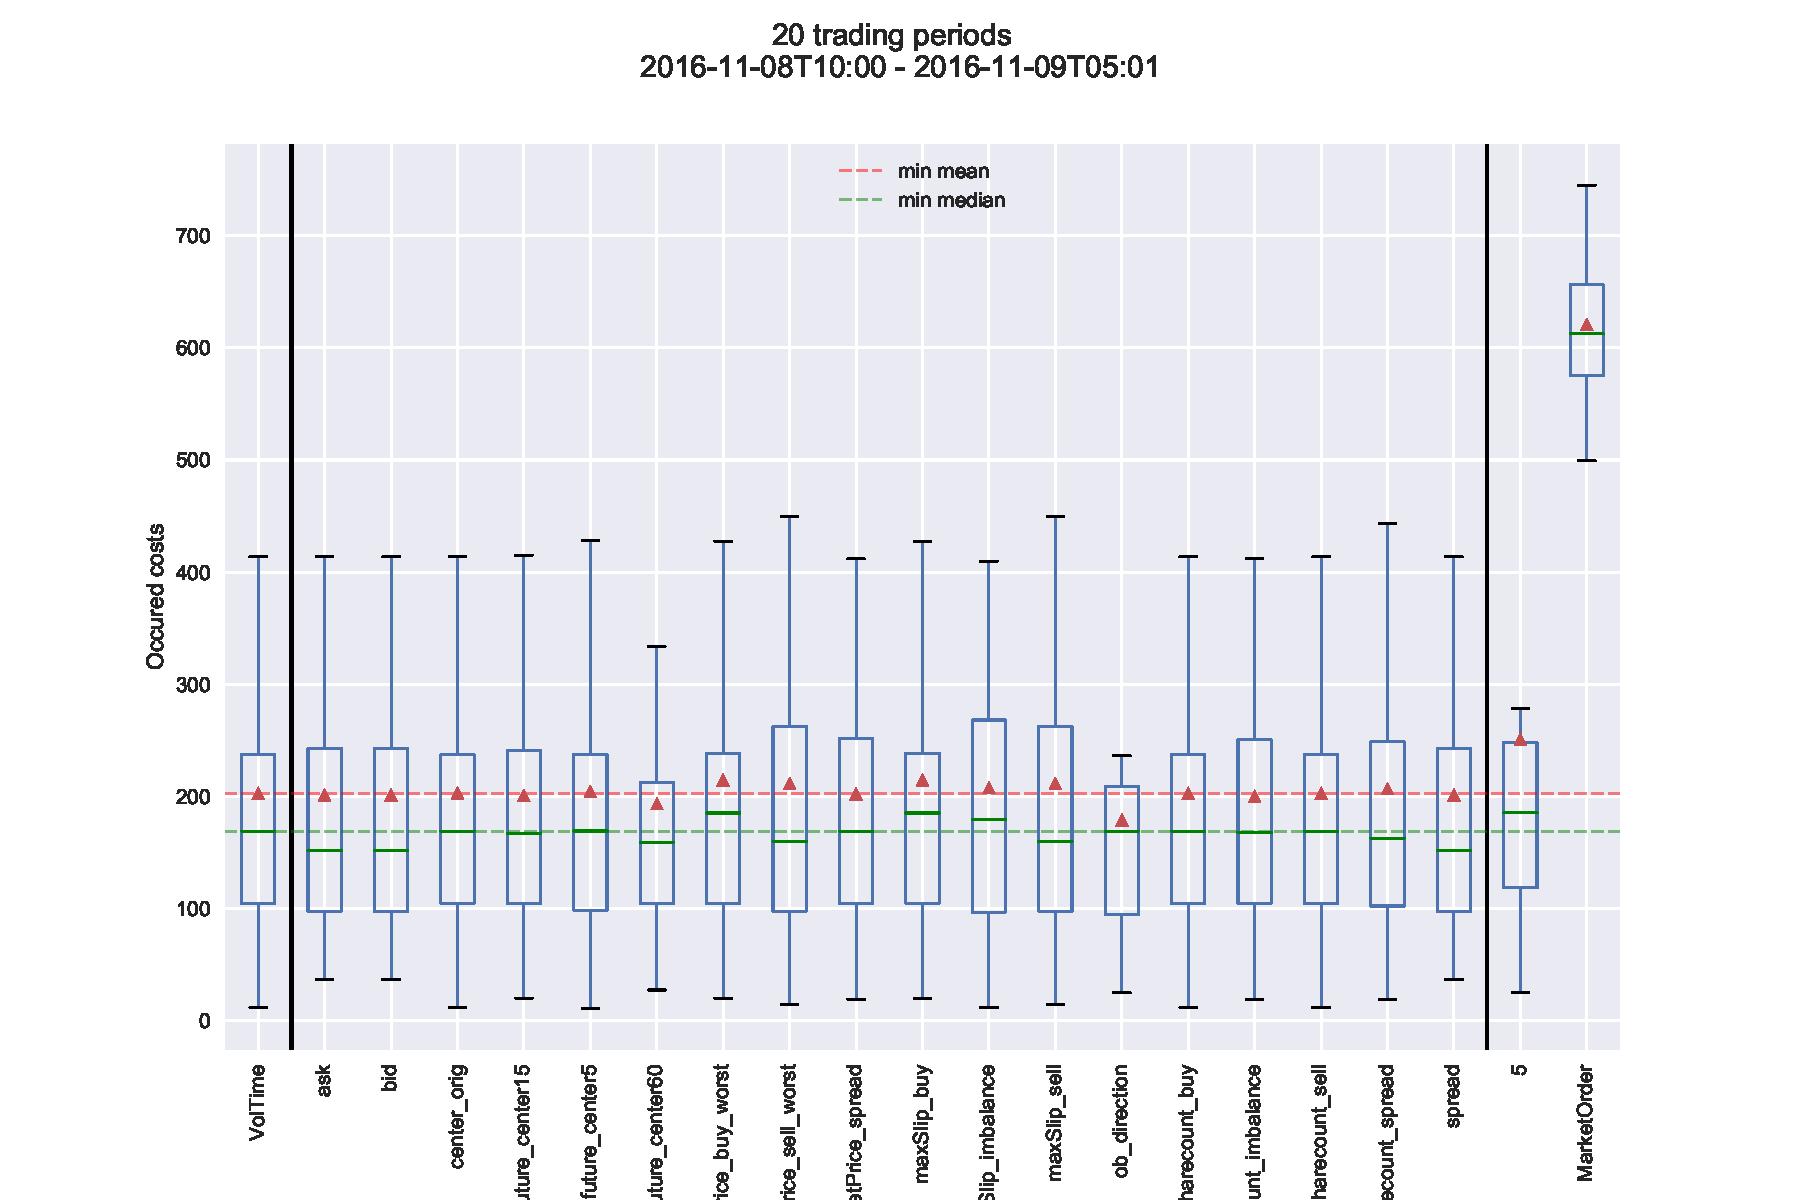
\includegraphics[width=\textwidth]{content/drawings/slippage_additionalMarketVars}
        		\caption{Slippage.}
		\label{fig:eval:additionalMarketVariables:plot}
    	\end{subfigure}%
	\begin{subfigure}[b]{0.25\textwidth}
        		\centering
		\scalebox{0.6}{
		\begin{tabular}{lr}
\toprule
{} &           mean slippage \\
\midrule
VolTime                &  202.737500 \\
ask                    &  201.214796 \\
bid                    &  201.214796 \\
center\_orig            &  202.737500 \\
future\_center15        &  200.865082 \\
future\_center5         &  204.489075 \\
future\_center60        &  193.398691 \\
marketPrice\_buy\_worst  &  214.750825 \\
marketPrice\_sell\_worst &  211.453516 \\
marketPrice\_spread     &  202.233493 \\
maxSlip\_buy            &  214.750825 \\
maxSlip\_imbalance      &  207.770109 \\
maxSlip\_sell           &  211.453516 \\
ob\_direction           &  179.040837 \\
sharecount\_buy         &  202.737500 \\
sharecount\_imbalance   &  200.049701 \\
sharecount\_sell        &  202.737500 \\
sharecount\_spread      &  206.764315 \\
spread                 &  201.214796 \\
5                      &  251.008681 \\
MarketOrder            &  620.867742 \\
\bottomrule
\end{tabular}}        		 
        		\caption{Mean slippage.}
		\label{fig:eval:additionalMarketVariables:mean}
    	\end{subfigure}

	\caption{Evaluating the impact of additional market variables.}
	\label{fig:eval:additionalMarketVariables}
\end{figure}




\section{Backward approach}

\subsection{QTable Agent + additional orderbook features}
bla

\subsection{QTable Agent + additional technical indicators}

\subsection{QTable Agent vs. BatchTree Agent vs. NN Agent}
bla




\section{Forward approach}
\label{chap:forwardlearning}
bla

\subsection{Motivation}
Markov Assumption is wrong: States do depend on path chosen before.

Data efficency. Learning with fewer samples

No need for discretization of volume.

\subsection{Results}
bla





\cleardoublepage{}